\documentclass[11pt,a4paper,polish,thesis,oneside]{dcsbook}

\usepackage[utf8]{inputenc}
\usepackage{babel}
\usepackage{indentfirst}
\usepackage{listings}
\usepackage{graphicx}

\setcounter{secnumdepth}{3}
\setcounter{tocdepth}{3}

\graphicspath{ {images/} }


\lstdefinelanguage{diff}{
  morecomment=[f][\color{blue}]{@@},     % group identifier
  morecomment=[f][\color{red}]-,         % deleted lines 
  morecomment=[f][\color{green}]+,       % added lines
  morecomment=[f][\color{magenta}]{---}, % Diff header lines (must appear after +,-)
  morecomment=[f][\color{magenta}]{+++},
}


\lstset{
    breaklines=true,
    postbreak=\raisebox{0ex}[0ex][0ex]{\ensuremath{\color{red}\hookrightarrow\space}}
}


\begin{document}

\author{inż.~Jakub Woźniak}
\title{Web Application Firewall}
\secondtitle{\textsc{Projekt i implementacja narzędzia testującego bezpieczeństwo reguł ModSecurity}}
\supervisor{dr inż.~Michał Szychowiak}
\date{Poznań, 2017}
\maketitle
\frontmatter
\tableofcontents
\mainmatter

% http://www.securityweek.com/evaluating-web-application-firewalls-things-keep-mind

\chapter{Wstęp}

Aplikacje internetowe (ang. \textit{web applications}) stopniowo wypierają ich okienkowe odpowiedniki. Przeglądarka internetowa stała się nieodłącznym elementem pracy przy komputerze. Popularność zyskują również systemy operacyjne, które opierają się wyłącznie o przeglądarkę i~przetwarzanie w chmurze. Wraz z upowszechnieniem się aplikacji internetowych, wzrosła również liczba ataków komputerowych, które mają na celu uzyskanie dostępu do prywatnych danych użytkowników lub zmuszenie ich do nieświadomego podjęcia jakiejś akcji. Baza danych \textit{Common Vulnerabilities and Exposures}\cite{cve} zawiera ponad 82 tysiące\footnote{stan na 17 marca 2017 r.} unikalnych, skatalogowanych podatności oprogramowania.

Dostępność otwartego i~rozbudowanego oprogramowania takiego jak Wordpress\cite{wordpress} czy Joomla\cite{joomla} połączona z dynamicznym rozwojem i~aktywnością społeczności programistów o różnym doświadczeniu stanowi poważny problem dla bezpieczeństwa tych aplikacji i~danych osób z nich korzystających. Wiele z odkrytych podatności znajduje się w~nieoficjalnych wtyczkach napisanych przez wolontariuszy i~udostępnionych na otwartych licencjach. Osoby zarządzające serwisami opartymi o ww. systemy często nie są świadome tych zagrożeń i~nie aktualizują oprogramowania na swoich serwerach. 

Dla samego systemu Wordpress w CVE skatalogowano ponad 290 podatności (statystyka nie dotyczy wtyczek), a~ostatnia z~nich opublikowana 11 marca 2017 roku dotyczy ataku typu CSRF\footnote{stan na 17 marca 2017 r.}, który pozwala na nadmierne wykorzystanie zasobów serwera (procesor, pamięć operacyjna), co w ostateczności może doprowadzić do ataku typu Denial of Service i~spowodowania niedostępności serwisu.

Również zamknięte i~komercyjne oprogramowanie nie jest wolne od błędów. Invision Power Board\cite{ipb} to komercyjny system pozwalający na prowadzenie forum dyskusyjnego. W bazie CVE znajduje się 11 odkrytych podatności\footnote{stan na 17 marca 2017 r.}, ostatnia jest z 12 lipca 2016 roku i~dotyczy możliwości zdalnego wykonania kodu na serwerze.

W styczniu 2017 roku w CVE skatalogowano 1085 podatności, znaczna część z nich dotyczyła bezpieczeństwa aplikacji internetowych. Były to m.in.\ ataki typu: XSS, SQL Injection, CSRF i zdalnego wykonania kodu. W przypadku otwartego oprogramowania społeczność zazwyczaj dość szybko reaguje na pojawiające się zagrożenia, pojawiają się aktualizacje bezpieczeństwa, które należy pobrać i~zainstalować na własnym serwerze. Zamknięte oprogramowanie wymaga reakcji producenta, co może wiązać się z długim czasem oczekiwania czy nawet negacją zagrożenia ze strony dostawcy.

Niestety nawet natychmiastowe wydanie aktualizacji przez producenta nie gwarantuje nam bezpieczeństwa. Aplikacje takie jak Wordpress czy Invision Power Board są utrzymywane i~zarządzane przez właściciela serwisu (np.\ przez nas samych). O podatności odkrytej w nocy możemy dowiedzieć się dopiero następnego dnia lub całkowicie przeoczyć taką informację. Crackerzy mogą spróbować zaatakować naszą stronę przy pomocy całkowicie nowego sposobu (zanim zostanie on upubliczniony, tzw. \textit{zero-day exploit}).

Powstała potrzeba posiadania zabezpieczenia podobnego do oprogramowania antywirusowego, które potrafi rozpoznawać zagrożenia bazując na znanych sygnaturach i~dodatkowo przeciwdziałać nieznanym atakom przy pomocy heurystyk. Takim odpowiednikiem jest Web Application Firewall, który występuje zarówno jako oprogramowanie pośredniczące instalowane na standardowych systemach operacyjnych, jak i~rozwiązania sprzętowe (np. wbudowane w urządzenia klasy UTM\footnote{Unified Threat Management}). WAF dokonuje analizy ruchu na 7.~warstwie modelu OSI i~zależnie od wyniku algorytmu oceniającego zagrożenie --- blokuje lub dopuszcza ruch z/do serwera www.  

\section*{Cel i zakres pracy}
Celem niniejszej pracy magisterskiej jest stworzenie narzędzia pozwalającego na automatyczne testowanie konfiguracji Web Application Firewall. Test ma polegać na przygotowaniu zestawu wektorów ataku, przeprowadzenie tego ataku na testowany WAF, a~następnie ocenę czy ruch sieciowy został poprawnie zablokowany. W celu przygotowania pracy magisterskiej należało dokonać analizy bieżących zagrożeń dotyczących aplikacji internetowych i~zapoznanie się z istniejącymi rozwiązaniami klasy WAF (w szczególności ModSecurity\cite{modsec}). Następnie wykonano prototypową realizację narzędzia testującego i~przeprowadzono testy konfiguracji na przygotowanym środowisku. Na podstawie wyników testów podjęto próbę przygotowania zestawu reguł, które pozwoliłyby na zablokowanie zagrożeń, które nie zostały wykryte przez WAF.

Struktura pracy jest następująca: TODO.


\chapter{Wprowadzenie teoretyczne}
Realizacja pracy wymagała zapoznania się z technologiami wykorzystywanymi przy tworzeniu aplikacji internetowych i potencjalnymi zagrożeniami bezpieczeństwa, na które są te aplikacje narażone.
\section{Zagrożenia aplikacji internetowych}
% OWASP TOP 10
Współczesne aplikacje internetowe są wielowarstwowe i wykorzystują różne technologie, m.in.~kod wykonywany po stronie klienta (JavaScript), kod wykonywany po stronie serwera (np.~PHP, Python, Ruby), bazy danych, itp.. Każda z tych technologii jest narażona na obecność podatności, które mogą być wykorzystane przez crackerów do wykradzenia informacji poufnych.

Internetowa społeczność \textbf{Open Web Application Security Project (OWASP)}\cite{owasp} zajmuje się tworzeniem artykułów, dokumentacji i narzędzi związanych z bezpieczeństwem sieci komputerowych. Jeden z ich największych projektów to \textbf{OWASP Top Ten}, którego celem jest podniesienie świadomości użytkowników na temat bezpieczeństwa aplikacji przez publikowane listy 10 najważniejszych zagrożeń. Poniżej zaprezentowano listę zagrożeń aplikacji internetowych wg \textbf{OWASP Top Ten 2017 Project}.

\subsection{Iniekcja kodu}
Iniekcja kodu to wykorzystanie błędu, który pozwala na przekazanie do wykonania niezaufanych danych wprowadzonych z zewnątrz. Potencjalnie narażona jest na to każda aplikacja w której użytkownik może wprowadzić dane. Atak polega na wprowadzeniu tekstu, który wykorzystuje składnię atakowanego interpretera, stąd jest on prosty do wykonania i bardzo skuteczny. Szczególnie narażone są następujące technologie: SQL, LDAP, XPath, NoSQL, polecenia systemu operacyjnego, parsery XML. itp.. Iniekcja może spowodować wyciek informacji, utratę danych (lub ich uszkodzenie), a w skrajnych przypadkach nawet całkowite przejęcie kontroli nad systemem.

Ochrona przed tym atakiem jest dość prosta, znaczna część bibliotek (np. do komunikacji z bazami danych) udostępnia mechanizmy pozwalające na separację wprowadzonych danych od składni interpretera (wiązanie zmiennych).

\subsubsection*{Przykład}
\begin{lstlisting}[language=php,frame=single,caption=kod podatny na iniekcję,label=injectionphp,numbers=left]
<?php

$id = $_GET["id"];
$query  = "SELECT id, name, price FROM products WHERE id = $id";
$result = pg_query($conn, $query);

?>
\end{lstlisting}
Zaprezentowany kod \ref{injectionphp} przyjmuje wartość parametru \textit{id} przekazaną przy pomocy URI przez użytkownika, a następnie zapisuje ją do zmiennej. Zmienna ta jest wykorzystana w zapytaniu SQL (linia 4). Brak weryfikacji zawartości tej zmiennej spowoduje wstawienie do zapytania dowolnego kodu przekazanego w parametrze. Jeżeli do zmiennej zostanie wprowadzona wartość \lstinline[frame=single]|4; DROP TABLE products; --|, to ostatecznie wykonane zapytanie będzie wyglądało następująco: 
\begin{lstlisting}
SELECT id, name, price FROM products WHERE id = 4; DROP TABLE products; --
\end{lstlisting}
Powyższe wykonanie spowoduje usunięcie z bazy danych relacji o nazwie \textit{products}.

Podatność na iniekcję kodu SQL wykryto np. w popularnym systemie zarządzania treścią JPortal (CVE-2007-5973). Pozwalała ona na wykonanie dowolnego kodu SQL przez parametr \textit{topic} w skrypcie \textit{articles.php}

\begin{lstlisting}[language=php,frame=single,caption=podatność articles.php w systemie JPortal,label=injectionjportal,numbers=left]
<?php

function topic_name($a)  
{     
global $topic_tbl; 
$query = "SELECT * FROM $topic_tbl WHERE id=$a"; 
$result = mysql_query($query);   
$r = mysql_fetch_array($result);     
return '<a href="articles.php?topic='.$a.'" class="t_main">'.$r['title'].'</a>';   
} 

?>
\end{lstlisting}

Przekazanie do parametru wartości \lstinline|-1+UNION+SELECT+1,pass,3,4,5+FROM+admins/| pozwalało na otrzymanie nazwy użytkownika i skrótu hasła (MD5 bez soli) kont z uprawnieniami administratora.
\subsection{Błędy uwierzytelnienia i zarządzania sesją}
Kolejnym popularnym zagrożeniem są błędy związane z uwierzytelnieniem użytkowników i zarządzaniem sesją. Dane związane z sesją (nazwa użytkownika, hasło, identyfikator sesji) są często przechowywane w sposób narażający na ujawnienie informacji --- brak funkcji skrótu lub szyfrowania, przesyłanie danych w formie czystego tekstu. Szczególnie ważny jest tutaj mechanizm, który rozpoznaje uprawnienia użytkownika podczas kolejnych, niezależnych żądań HTTP. Często wiele z tych danych jest przechowywanych w postaci ciasteczka \textit{(ang. cookie} po stronie przeglądarki, jego przechwycenie lub modyfikacja może spowodować przejęcie konta ofiary lub eskalację uprawnień.

W nowszych systemach, użytkownik w ciasteczku otrzymuje wyłącznie informacje o identyfikatorze sesji, a dane z nią związane przechowywane są po stronie serwera. Takie rozwiązanie jest również podatne na atak fiksacji sesji. Jeżeli weryfikowany jest tylko identyfikator sesji, to przechwycenie tego identyfikatora powoduje przejęcie sesji. Potencjalnie zagrożone są aplikacje:
\begin{itemize}
\item przechowują identyfikator sesji w adresie URI,
\item nie regenerują identyfikatora przy logowaniu,
\item nie korzystają z mechanizmu wygasania sesji po określonym czasie,
\item nie weryfikują innych danych żądania poza identyfikatorem (np. adresu IP czy sygnatury przeglądarki),
\item przesyłają informacje nieszyfrowanym kanałem.
\end{itemize}

\subsubsection*{Przykład}
Załóżmy istnienie sklepu internetowego, który przechowuje identyfikator sesji w URI. Zalogowany użytkownik \textit{A} przegląda stronę i chce pokazać ofertę innej osobie, więc kopiuje z przeglądarki adres strony o następującej postaci:
\begin{lstlisting}
http://example.com/sklep/oferta.php?sessid=5aef77ef7aa
\end{lstlisting}
Użytkownik \textit{B} po wejściu na otrzymany adres będzie zalogowany z uprawnieniami użytkownika \textit{A} i otrzyma dostęp do wszystkich informacji o tym użytkowniku, które są przechowywane w systemie.

Innym, bardziej prawdopodobnym atakiem jest przekazanie ofierze adresu z spreparowanym identyfikatorem sesji. Jeżeli aplikacja nie regeneruje identyfikatora po zalogowaniu, to atakujący będzie mógł przejąć sesję, jeśli ofiara zaloguje się przy pomocy przekazanego adresu. Na taki atak był podatny system CMS Symphony2 (CVE-2016-4309). Przy błędnie skonfigurowanym interpreterze języka PHP (brak wymuszenia przechowywania identyfikatora sesji w ciasteczku) atakujący mógł wymusić konkretny identyfikator sesji przy pomocy parametru \textit{PHPSESSID} przekazanego w URI. Stosowna poprawka pojawiła się w repozytorium projektu i usunęła wskazaną podatność (przykład \ref{symphonydiff}).

\begin{lstlisting}[language=diff,frame=single,caption=łatka naprawiająca podatność fiksacji sesji w Symphony2 \cite{symphony},label=symphonydiff,numbers=left]
diff --git a/symphony/lib/core/class.session.php b/symphony/lib/core/class.session.php
index c0075a1..dedb526 100644
--- a/symphony/lib/core/class.session.php
+++ b/symphony/lib/core/class.session.php
@@ -58,6 +58,9 @@ public static function start($lifetime = 0, $path = '/', $domain = null, $httpOn
 
             if (session_id() == '') {
                 ini_set('session.save_handler', 'user');
+                ini_set('session.use_trans_sid', '0');
+                ini_set('session.use_strict_mode', '1');
+                ini_set('session.use_only_cookies', '1');
                 ini_set('session.gc_maxlifetime', $lifetime);
                 ini_set('session.gc_probability', '1');
                 ini_set('session.gc_divisor', Symphony::Configuration()->get('session_gc_divisor', 'symphony'));
\end{lstlisting}

\subsection{Cross-site scripting (XSS)}
\textit{Cross-Site Scripting} (XSS) to sposób ataku na aplikację internetową, który polega na możliwości osadzenia kodu JavaScript w treści strony internetowej w taki sposób, by był on wykonany po stronie przeglądarki ofiary ataku. Atak ten jest możliwy jeżeli aplikacja zmienia zawartość strony internetowej na podstawie danych wprowadzonych z zewnątrz (np. parametry GET/POST) bez uprzedniej zamiany znaków specjalnych HTML na encje. 

Wyróżnia się dwa rodzaje ataku XSS:
\begin{itemize}
\item persistent XSS --- kiedy kod zostaje zapamiętany przez aplikację internetową i jest wyświetlony każdemu odwiedzającemu,
\item non-persistent XSS --- kiedy kod jest dostępny tylko w odpowiedzi na konkretne żądanie HTTP.
\end{itemize}

Wykonanie dowolnego kodu JavaScript po stronie przeglądarki ofiary może mieć następujące skutki:
\begin{itemize}
\item przejęcie sesji użytkownika lub innych danych przechowywanych w ciasteczkach,
\item podmiana zawartości strony internetowej (np. numerów kont bankowych do przelewu),
\item przekierowanie użytkownika na inną stronę,
\item pobranie złośliwego oprogramowania,
\item przesłanie zawartości strony (np. danych osobowych) na inny serwer.
\end{itemize}

\subsubsection*{Przykład}
Przykład \ref{xss1} zawiera kod strony podatnej na atak XSS. W ciasteczku przechowywana jest wartość \textit{secret=password}. Następnie na stronie wyświetla się napis \textit{Hello <var>}, gdzie \textit{var} to parametr przekazany w URL.

\begin{lstlisting}[language=php,frame=single,caption=przykładowy kod strony podatnej na XSS,label=xss1,numbers=left]
<?php

setcookie("secret", "password");
echo "<h1>Hello ".$_GET["name"]."</h1>";

?>
\end{lstlisting}

Przekazanie kodu \ref {xss2} w postaci parametru \textit{name} spowoduje wykonanie tego kodu po stronie przeglądarki. Efektem wywołania będzie przekierowanie użytkownika na adres internetowy z przekazaną zawartością ciasteczka w adresie URL.

\begin{lstlisting}[language=php,frame=single,caption=przykład wykorzystania podatności XSS,label=xss2,numbers=left]
<script>document.location="http://example.com/?c="+document.cookie;</script>

%3Cscript%3Edocument.location%3D%22http%3A%2F%2Fexample.com%2F%3Fc%3D%22%2Bdocument.cookie%3B%3C%2Fscript%3E (wersja zakodowana)
\end{lstlisting}

W 2014 roku odkryto podatność aplikacji TweetDeck \cite{tweetdeck} (działającej jako rozszerzenie do przeglądarki Google Chrome), która oferowała interakcję z popularnym serwisem społecznościowym Twitter. Podatność polegała na renderowaniu treści tweeta z wykorzystaniem silnika interpretującego JavaScript i bez zamiany danych pobranych z API na encje.

\begin{figure}[h]
\centering
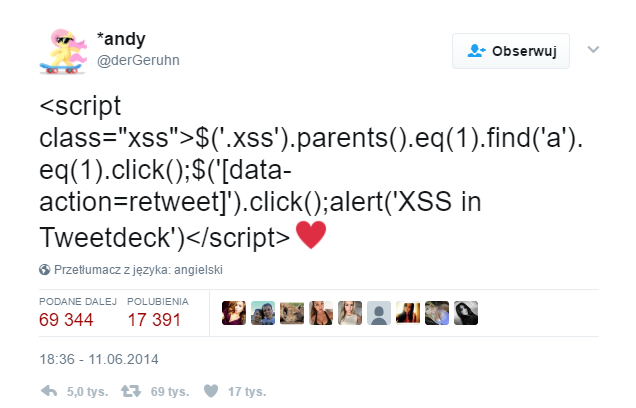
\includegraphics[scale=0.75]{tweetdeck}
\label{tweetdeckpng}
\caption{tweet wykorzystujący podatność XSS w TweetDeck}
\end{figure}

Użytkownik \textit{@derGeruhn} zamieścił na swoim profilu wpis, który wykorzystywał odnalezioną podatność. Wyświetlony w aplikacji TweetDeck zawierał tylko emotikonę serca, a poprzedzający ją kod został wykonany z uprawnieniami ofiary. Zamieszczony kod powodował rozpowszechnienie wpisu przez skopiowanie go na profil ofiary (\textit{ang. retweet}). Próba usunięcia wpisu kończyła się pojawieniem się komunikatu ,,XSS in Tweetdeck''.

\subsection{Błędna kontrola dostępu do obiektu}
Ataki wykorzystujące błędną kontrolę dostępu do obiektu polegają na podmianie parametrów autoryzujących lub bezpośrednie wywołanie niepublicznych funkcji, do których dostęp nie jest odpowiednio weryfikowany. Jest to szczególnie ważne przy projektowaniu publicznych API, gdzie URL często zawiera nazwy obiektów. Przez modyfikowanie tej nazwy można odwołać się do obiektu, do którego nie mamy dostępu. Jest to podatność prosta do wykrycia, niestety jej obecność może umożliwić ujawnienie poufnych danych zgromadzonych w systemie.

\subsubsection*{Przykład}
Kod (przykład \ref{da01}) odpowiada za pobranie wiadomości prywatnych użytkownika. Załóżmy, że funkcja \textit{LookupMessageObject} weryfikuje czy dane są numeryczne, a wiadomości są składowane w jednym miejscu (niezależnie od użytkownika), identyfikowane wyłącznie wg identyfikatora tej wiadomości. Kod aplikacji prawidłowo sprawdza czy użytkownik jest zalogowany. Wywołanie funkcji \textit{DisplayPrivateMessage} nie weryfikuje uprawnień zalogowanego użytkownika do żądanej wiadomości. Każdy zalogowany użytkownik może modyfikując parametr \textit{id} próbować pobrać dowolną wiadomość (zakładając sekwencyjne przydzielanie identyfikatora jest to bardzo proste) z pozytywnym skutkiem.

\begin{lstlisting}[language=perl,frame=single,caption=przykładowy kod podatny na bezpośrednie odwołanie \cite{directaccess},label=da01,numbers=left]
sub DisplayPrivateMessage {
my($id) = @_;
my $Message = LookupMessageObject($id);
print "From: " . encodeHTML($Message->{from}) . "<br>\n";
print "Subject: " . encodeHTML($Message->{subject}) . "\n";
print "<hr>\n";
print "Body: " . encodeHTML($Message->{body}) . "\n";
}

my $q = new CGI;
# For purposes of this example, assume that CWE-309 and
# CWE-523 do not apply.
if (! AuthenticateUser($q->param('username'), $q->param('password'))) {
ExitError("invalid username or password");
}

my $id = $q->param('id');
DisplayPrivateMessage($id);
\end{lstlisting}

W 2015 roku odkryto wiele podatności w rozszerzeniu dla systemu Wordpress --- TheCartPress (CVE-2015-3300) \cite{thecartpress}. Jedna z nich polegała na błędnej kontroli dostępu do obiektu. Atakujący mógł otworzyć następujący URL [\ref{thecartpress1}], a następnie przejść na adres [\ref{thecartpress2}], który zawiera pełne informacje dotyczące zamówienia w sklepie internetowym. Identyfikator zamówienia jest inkrementacją poprzedniej wartości, stąd łatwo przewidzieć dozwolone wartości i otrzymać pełne informacje o wszystkich zamówieniach w systemie.

\begin{lstlisting}[caption=adres URL zamówienia w systemie TheCartPress,label=thecartpress1]
http://wordpress/shopping-cart/checkout/?tcp_checkout=ok&order_id=[order_id]
\end{lstlisting}

\begin{lstlisting}[caption=adres URL przeznaczony dla administratora do podglądu zamówienia,label=thecartpress2]
http://wordpress/wp-admin/admin-ajax.php?order_id=[order_id]&action=tcp_print_order
\end{lstlisting}


\subsection{Błędna konfiguracja bezpieczeństwa}
Błędy związane z konfiguracją bezpieczeństwa mogą wystąpić praktycznie na każdej warstwie aplikacji: sprzęt, system operacyjny, serwer WWW, system zarządzania bazą danych, kod źródłowy. Szczególną uwagę należy zwrócić na aktualizacje bezpieczeństwa, które łatają podatności oprogramowania wykorzystywanego na serwerze. Ważnym elementem jest również prawidłowa konfiguracja zapory sieciowej i udostępnienie tylko potrzebnych usług. Gotowe aplikacje internetowe często posługują się domyślnym kontem administratora, które ma powszechnie znane hasło. Takie konta należy dezaktywować, ponieważ nawet zautomatyzowane ataki wykorzystują te dane do prób włamania. Również przy tworzeniu własnego oprogramowania można popełnić wiele błędów. Platformy programistyczne (\textit{ang. framework}) często udostępniają tryb debugowania, który podczas błędów udziela szczegółowych informacji o wystąpieniu problemu (nawet z fragmentami kodu). Pozostawienie takiego trybu na systemach produkcyjnych może spowodować wyciek informacji o architekturze systemu i wartości sekretnych zmiennych.

\subsubsection*{Przykład}
Django \cite{django} to framework dla języka Python, który pozwala na tworzenie aplikacji internetowych. Na szczególną uwagę zasługują dwie zmienne środowiskowe w pliku konfiguracyjnym: \textit{DEBUG} i \textit{SECRET\_KEY}. Główną funkcją zmiennej \textit{DEBUG} jest szczegółowy widok błędu. Gdy aplikacja napotka na błąd wykonania (nieprzechwycony wyjątek) to wyświetli dokładny opis problemu, wraz z fragmentami kodu na stosie wywołań, zawartością plików konfiguracyjnych i treścią żądania HTTP. W celu zwiększenia bezpieczeństwa, twórcy Django dodali automatyczne usuwanie wartości zmiennych o nazwach podobnych do ,,pass'', ,,token'', itp. W połączeniu z dodatkowymi rozszerzeniami, programista może w łatwy sposób uzyskać interaktywną konsolę z interpreterem języka Python, która będzie działała na stronie ze szczegółami błędu. Uruchomienie aplikacji w tym trybie na systemie produkcyjnym pozwoli atakującemu w łatwy sposób przejąć kontrolę nad powłoką systemową i wykonać dowolne polecenia. Zmienna \textit{SECRET\_KEY} służy do podpisów kryptograficznych i powinna być unikalna oraz nieprzewidywalna. Częstym błędem jest niezmienianie wartości tej zmiennej po pobraniu projektu, przez co atakujący może podpisać własne dane przy pomocy znanego klucza, a aplikacja zaakceptuje je i np.~autoryzuje użytkownika.

W 2009 roku znany portal internetowy wykop.pl został zaatakowany, czego skutkiem był wyciek bazy danych serwisu wraz z danymi o użytkownikach (nazwy, skróty haseł bez soli, adresy e-mail) \cite{wykop}. Baza danych przeznaczona do celów deweloperskich (zawierające kopię bazy produkcyjnej z zachowaniem oryginalnych danych) była dostępna publicznie, bez weryfikacji adresu IP klienta, a sama usługa działała na domyślnych ustawieniach --- brak hasła dla użytkownika \textit{root}. Atakujący w łatwy sposób uzyskali pełną kontrolę nad usługą bazy danych i skopiowali składowane tam informacje.

\subsection{Ujawnienie wrażliwych danych}
Przy projektowaniu aplikacji internetowej należy mieć na uwadze możliwość uzyskania przez atakującego dostępu do składowanych danych lub kopii zapasowych tych danych. Jest to możliwe na wszystkich etapach komunikacji sieciowej --- dostęp do danych składowanych na serwerze, podsłuchanie ruchu sieciowego, uzyskanie informacji z przeglądarki internetowej ofiary. Algorytmy kryptograficzne są ciężkie do złamania, dlatego atakujący skupiają się na słabych elementach systemu: kradzież kluczy kryptograficznych, atak typu man-in-the-middle, pozyskanie danych w postaci czystego tekstu po deszyfrowaniu wiadomości przez serwer.

Szczególnie wrażliwe dane to: hasła użytkowników, dane osobowe, numery kart kredytowych, itp. Zagrożeniem dla aplikacji jest przechowywanie lub przesyłanie tych danych w postaci czystego tekstu. Jeżeli wprowadzono mechanizmy kryptograficzne, to należy zadbać o dobranie silnych algorytmów i kluczy kryptograficznych (którymi należy odpowiednio zarządzać i rotować co określony czas). Wciąż popularne jest przechowywanie haseł użytkowników w formie skrótu MD5 lub SHA1 bez wprowadzonego ciągu zaburzającego (tzw.~soli). Korzystanie z tych algorytmów jest niezalecane, ponieważ stosunkowo łatwo jest odnaleźć pierwotną formę hasła (nawet przy pomocy ataków typu \textit{brute force}). 

Dane przesyłane przy pomocy protokołu HTTP powinny być również szyfrowane, służy do tego protokół TLS. Do ustalenia bezpiecznego kanału komunikacji wykorzystuje się certyfikaty X.509. Współcześnie uzyskanie takiego certyfikatu jest bardzo proste. Projekt Let's Encrypt zarządzany przez Internet Security Research Group ma na celu upowszechnienie stosowania protokołu HTTPS. Jest to urząd certyfikacji, który oferuje darmowe certyfikaty X.509. Dzięki temu można w prosty sposób zapewnić podstawowe bezpieczeństwo komunikacji bez ponoszenia dodatkowych kosztów.

\subsubsection*{Przykład}
W czerwcu 2016 roku największy rosyjski portal społecznościowy VK.com został zaatakowany \cite{vk}. W wyniku ataku uzyskano dostęp do bazy danych serwisu, która zawierała dane osobowe użytkowników, adresy e-mail oraz hasła przechowywane w formie czystego tekstu. Kopia bazy zawierała ponad 100 milionów rekordów. Było to szczególnie niebezpieczne dla tych użytkowników, którzy korzystali z tego samego hasła również w innych serwisach internetowych. 


\subsection{Niewystarczająca ochrona przed atakami}
Zabezpieczenie się przed wszystkimi rodzajami ataków jest bardzo trudne do zrealizowania. Niektóre z nich nie wykorzystują podatności samej aplikacji, a np.~próbują w zautomatyzowany sposób odgadnąć hasła użytkowników metoda siłową. W celu zwiększenia bezpieczeństwa należy wdrożyć mechanizmy wykrywania i reagowania na ataki (manualne i zautomatyzowane).

Detekcja ataków polega na monitorowaniu przychodzącego ruchu sieciowego (również na warstwie aplikacji) i analizie pod kątem: częstotliwości żądań, wprowadzanych danych, powtarzalności, itp. Nawet podstawowa metryka polegająca na analizie wolumenu ruchu per adres IP pozwala na wykrycie anomalii i podjęcie odpowiedniej reakcji. Reagowanie na ataki to przede wszystkim powiadomienie administratorów o zaistniałym potencjalnym zagrożeniu. Na podstawie rejestrów zdarzeń można podjąć decyzję o zablokowaniu danego adresu IP lub całego zakresu. W przypadku uwierzytelnionych użytkowników jedną z możliwości jest zablokowanie konta użytkownika.

Odnalezione podatności wymagają wytworzenia przez programistów odpowiedniej aktualizacji. W przypadku zewnętrznego oprogramowania, proces ten może potrwać nawet kilka tygodni. W tym celu można wykorzystać mechanizmy, które analizują ruch HTTP i blokują określone wzorce żądań wykorzystujące podatności aplikacji.

\subsubsection*{Przykład}
Jednym z popularnych mechanizmów do obrony przed atakami siłowymi jest mechanizm \textit{CAPTCHA}. Polega on na wyświetleniu przy np. trzeciej i każdej kolejnej nieudanej próbie pewnego dodatkowego zadania, które użytkownik musi wykonać. Zazwyczaj polega to na przepisaniu frazy z wyświetlonego obrazu, który jest przygotowany w taki sposób, by utrudnić pracę algorytmom OCR. 


\subsection{Cross-site request forgery (CSRF)}
Jest to metoda ataku na aplikację internetową, która polega na wykorzystaniu przez atakującego uprawnień ofiary do nieświadomego wykonania przez nią określonej operacji. Atak ten jest często wykorzystywany razem z XSS.


\subsection{Korzystanie z komponentów o znanych podatnościach}
\subsection{Brak weryfikacji przekierowań}

\section{Mechanizmy wbudowane w przeglądarki internetowe}


\section{Web Application Firewall}
\label{waf}
Web Application Firewall to...

\subsection{Oprogramowanie}
\subsubsection{ModSecurity}
\subsubsection{NAXSI}

\subsection{Urządzenia}
\subsubsection{Citrix Netscaller Application Firewall}
\subsubsection{Fortinet FortiWeb}

\subsection{Rozwiązania chmurowe}
\subsubsection{Amazon Web Services WAF}
\subsubsection{Cloudflare}

\section{Intrusion Prevention System}

\chapter{Implementacja systemu}

\chapter{Testy funkcjonalne}


\chapter{Zakończenie}

\backmatter

\begin{thebibliography}{1}
\bibitem{cve} Common Vulnerabilities and Exposures, https://cve.mitre.org/ [dostęp: 17 marca 2017]
\bibitem{wordpress} https://wordpress.org/
\bibitem{joomla} https://www.joomla.org/
\bibitem{ipb} https://invisionpower.com/
\bibitem{modsec} https://modsecurity.org/
\bibitem{owasp} https://www.owasp.org/
\bibitem{symphony} https://github.com/symphonycms/symphony-2/commit/b329a14adc40868965076a77210452e396243dcd.diff
\bibitem{tweetdeck} http://www.businessinsider.com/tweetdeck-major-security-vulnerability-twitter-2014-6 [dostęp 03.05.2017 r.]
\bibitem{directaccess} https://cwe.mitre.org/data/definitions/285.html
\bibitem{thecartpress} https://www.htbridge.com/advisory/HTB23254 [dostę:p 06.05.2017 r.]
\bibitem{django} https://www.djangoproject.com/
\bibitem{wykop} http://prawo.vagla.pl/node/8629 [dostęp: 06.05.2017 r.]
\bibitem{vk} http://thehackernews.com/2016/06/vk-com-data-breach.html [dostęp: 07.05.2017 r.]

\end{thebibliography}

\end{document}
